\documentclass[11pt,letterpaper]{article}


% pmml  arff  openannotation

%\usepackage[condensed,math]{anttor}
%\usepackage[T1]{fontenc}

%\usepackage[T1]{fontenc}
%\usepackage{tgtermes}

\usepackage[hang,flushmargin]{footmisc}

\usepackage{titlesec}

%\usepackage{sectsty}
%\sectionfont{\fontsize{13}{4}\selectfont}

\titleformat{\section}
  {\normalfont\fontsize{13}{15}\bfseries}{\thesection}{1em}{}

\let\OldPart\part

\renewcommand{\part}[1]{\OldPart{#1}%
%{\textcolor{darkRed}\hrule}
\vspace{-.5em}}

\titlespacing*{\section}
{0pt}{4.1ex plus 1ex minus .1ex}{-0.2ex plus .2ex}

\titlespacing*{\subsection}
{0pt}{3.1ex plus 1ex minus .1ex}{-.8ex plus .2ex}

%\usepackage{mathptmx}

\usepackage{eso-pic}

%\setlength\parindent{0pt}

\AddToShipoutPictureBG{%

\ifnum\value{page}>1{
\AtTextUpperLeft{
\makebox[20.5cm][r]{
\raisebox{-2.45cm}{%
{\transparent{0.3}{
\includegraphics[width=0.29\textwidth]{e-logo.png}}	}} } }
}\fi
}

\AddToShipoutPicture{%
{
 {\color{blGreen!70!red}\transparent{0.9}{\put(0,0){\rule{3pt}{\paperheight}}}}%
 {\color{darkRed!70!purple}\transparent{1}\put(3,0){{\rule{4pt}{\paperheight}}}}
% {\color{logoPeach!80!cyan}\transparent{0.5}{\put(0,700){\rule{1cm}{.6cm}}}}%
% {\color{darkRed!60!cyan}\transparent{0.7}\put(0,706){{\rule{1cm}{.6cm}}}}
% \put(18,726){\thepage}
% \transparent{0.8}
}
}

\AddToShipoutPicture{%
\ifnum\value{page}=1
\put(257.5,942){%
	\transparent{0.7}{
		
\includegraphics[width=0.2\textwidth]{logo.png}}}
\put(59,953){\textbf{{\fontfamily{phv}\fontsize{14}{14}\selectfont{}WHITE PAPER}}}
\fi
}	



\AddToShipoutPicture{%
\ifnum\value{page}>1
{\color{blGreen!70!red}\transparent{0.9}{\put(300,6){\rule{0.5\paperwidth}{.3cm}}}}%
{\color{inOne}\transparent{0.8}{\put(300,8){\rule{0.5\paperwidth}{.3cm}}}}%
{\color{inTwo}\transparent{0.3}\put(300,11){{\rule{0.5\paperwidth}{.3cm}}}}

\put(301,14){%
\transparent{0.7}{

\includegraphics[width=0.2\textwidth]{logo.png}}
}
%\fi

%\pgfmathparse{equal(\value{page},15)||equal(\value{page},20)?int(1):int(0)}

\ifnum\value{page}=10   %\pgfmathresult>0\relax
\put(232,253.5){
 {\setlength{\fboxsep}{.65em}\fontsize{9}{10}\selectfont

   {\color{white}{\parbox{11cm}{\vspace{7pt}{\begin{minipage}{.46\textwidth}
	  {\color{black}{\textit{For more information please contact:}}\\\textbf{\color{blGreen!40!blbl}{Amy Neustein, Ph.D., Founder and CEO}}\\  
       \textbf{{\color{blGreen!20!black}Linguistic Technology Systems \\
      amy.neustein@verizon.net \textbullet{} \textbf{(917) 817-2184} }}}
	 \end{minipage}}}}}}
}
\fi

{\color{blGreen!70!red}\transparent{0.9}{\put(5.6,3){\rule{0.5\paperwidth}{.4cm}}}}%
{\color{inOne}\transparent{1}{\put(5.6,8){\rule{0.5\paperwidth}{.4cm}}}}%
{\color{inTwo}\transparent{0.3}\put(5.6,13){{\rule{0.5\paperwidth}{.4cm}}}}

\fi
}

%\pagestyle{empty} % no page number
%\parskip 7.2pt    % space between paragraphs
%\parindent 12pt   % indent for new paragraph
%\textwidth 4.5in  % width of text
%\columnsep 0.8in  % separation between columns

%\setlength{\footskip}{7pt}

\usepackage[paperheight=14in,paperwidth=8.5in]{geometry}
\geometry{left=.72in,top=.39in,right=.68in,bottom=1.14in} %margins

\usepackage{etoolbox}% http://ctan.org/pkg/etoolbox
\makeatletter
% \patchcmd{<cmd>}{<search>}{<replace>}{<success>}{<failure>}
\patchcmd{\@part}{\par}{\quad}{}{}
\patchcmd{\@part}{\huge}{\Large}{}{}
\makeatother

\renewcommand{\partname}{\hspace{-1em}Part}

\renewcommand*\thepart{\Roman{part}:}

\renewcommand{\thepage}{\raisebox{2pt}{\arabic{page}}}

\renewcommand{\footnoterule}{%
	\kern 2pt
	\hrule width .92\textwidth height .5pt
	\kern 6pt
}


\usepackage[hyphens]{url}
\newcommand{\biburl}[1]{ {\fontfamily{gar}\selectfont{\textcolor[rgb]{.2,.6,0}%
{\scriptsize {\url{#1}}}}}}

%\linespread{1.3}

\newcommand{\sectsp}{\vspace{12pt}}

\usepackage{graphicx}
\usepackage{color,framed}

\usepackage{textcomp}

\usepackage{float}

\usepackage{mdframed}


\usepackage{setspace}
\newcommand{\rpdfNotice}[1]{\begin{onehalfspacing}{

\Large #1

}\end{onehalfspacing}}

\usepackage{xcolor}

\usepackage[hyphenbreaks]{breakurl}
\usepackage[hyphens]{url}

\usepackage{hyperref}
%\newcommand{\rpdfLink}[1]{\href{#1}{\small{#1}}}
%\newcommand{\dblHref}[1]{\href{#1}{\small{\burl{#1}}}}
%\newcommand{\browseHref}[2]{\href{#1}{\Large #2}}

\colorlet{blCyan}{cyan!50!blue}

\definecolor{darkRed}{rgb}{.2,.0,.1}


\definecolor{blGreen}{rgb}{.2,.7,.3}

\definecolor{darkBlGreen}{rgb}{.1,.3,.2}

\definecolor{oldBlColor}{rgb}{.2,.7,.3}

\definecolor{blColor}{rgb}{.1,.3,.2}

\definecolor{elColor}{rgb}{.2,.1,0}
\definecolor{flColor}{rgb}{0.7,0.3,0.3}

\definecolor{logoOrange}{RGB}{108, 18, 30}
\definecolor{logoGreen}{RGB}{85, 153, 89}
\definecolor{logoPurple}{RGB}{200, 208, 30}

\definecolor{logoBlue}{RGB}{4, 2, 25}
\definecolor{logoPeach}{RGB}{255, 159, 102}
\definecolor{logoCyan}{RGB}{66, 206, 244}
\definecolor{logoRed}{rgb}{.3,0,0}

\newcommand{\colorq}[1]{{\color{logoOrange!70!black}{\q{\small\textbf{#1}}}}}

\definecolor{inOne}{rgb}{0.122, 0.435, 0.698}% Rule colour
\definecolor{inTwo}{rgb}{0.122, 0.698, 0.435}% Rule colour

\definecolor{outOne}{rgb}{0.435, 0.698, 0.122}% Rule colour
\definecolor{outTwo}{rgb}{0.698, 0.435, 0.122}% Rule colour

\colorlet{linkcolor}{flColor!60!red}


\hypersetup{
	colorlinks=true,
	citecolor=blCyan!40!green,
	filecolor=magenta!30!logoBlue,
	urlcolor=blue,
    linkcolor=linkcolor!70!black,
%    allcolors=blCyan!40!green
}


\usepackage[many]{tcolorbox}% http://ctan.org/pkg/tcolorbox

\usepackage{transparent}

\newlength{\bsep}
\setlength{\bsep}{-1pt}
\let\xbibitem\bibitem
\renewcommand{\bibitem}[2]{\vspace{\bsep}\xbibitem{#1}{#2}}

\newenvironment{cframed}{\begin{mdframed}[linecolor=logoPeach,linewidth=0.4mm]}{\end{mdframed}}

\newenvironment{ccframed}{\begin{mdframed}[backgroundcolor=logoGreen!5,linecolor=logoCyan!50!black,linewidth=0.4mm]}{\end{mdframed}}


%\usepackage[T1]{fontenc}

%\usepackage{aurical}
% \Fontauri

\usepackage{gfsdidot}
\usepackage[T1]{fontenc}

%\makeatletter
%\f@family,  cmr, T1, n, m,
%\f@encoding,
%\f@shape,
%\f@series,
%\makeatother



%\usepackage{LibreBodoni}

%\usepackage{fontspec}
%\setmainfont{QTBengal}

\usepackage{relsize}

%
%\newcommand{\bref}[1]{\hspace*{1pt}\textbf{\ref{#1}}}

\newcommand{\bref}[1]{\hspace*{1pt}\textbf{\ref{#1}}}

\newcommand{\pseudoIndent}{

\vspace{10pt}\hspace*{12pt}}

\newcommand{\YPDFI}{{\fontfamily{fvs}\selectfont YPDF-Interactive}}

%
\newcommand{\deconum}[1]{{\protect\raisebox{-1pt}{{\LARGE #1}}}}

\newcommand{\visavis}{vis-\`a-vis}

\newcommand{\VersatileUX}{{\color{red!85!black}{\Fontauri Versatile}}%
{{\fontfamily{qhv}\selectfont\smaller UX}}}

\newcommand{\NDPCloud}{{\color{red!15!black}%
{\fontfamily{qhv}\selectfont {\smaller NDP C{\smaller LOUD}}}}}

\newcommand{\MThreeK}{{\color{blGreen!45!black}%
{\fontfamily{qhv}\fontsize{10}{8}\selectfont {M3K}}}}


\newcommand{\lfNDPCloud}{{\color{red!15!black}%
{\fontfamily{qhv}\selectfont N{\smaller DP C{\smaller LOUD}}}}}

\newcommand{\textds}[1]{{\fontfamily{lmdh}\selectfont{%
\raisebox{-1pt}{#1}}}}

\newcommand{\dsC}{{\textds{ds}{\fontfamily{qhv}\selectfont \raisebox{-1pt}
{\color{red!15!black}{C}}}}}

\definecolor{tcolor}{RGB}{24,52,61}

\newcommand{\CCpp}{\resizebox{!}{7pt}{\AcronymText{C}}/\Cpp{}}
\newcommand{\NoSQL}{\resizebox{!}{7pt}{\AcronymText{NoSQL}}}
\newcommand{\SQL}{\resizebox{!}{7pt}{\AcronymText{SQL}}}

\newcommand{\SPARQL}{\resizebox{!}{7pt}{\AcronymText{SPARQL}}}

\newcommand{\NCBI}{\resizebox{!}{7pt}{\AcronymText{NCBI}}}

\newcommand{\HTXN}{\resizebox{!}{7pt}{\ATexttclr{HTXN}}}

\newcommand{\sHTXN}{\resizebox{!}{6pt}{\ATexttclr{HTXN}}}

\newcommand{\TDM}{\resizebox{!}{7pt}{\AcronymText{TDM}}}

\newcommand{\lHTXN}{\resizebox{!}{7.5pt}{\ATexttclr{H}}%
\resizebox{!}{6.5pt}{\ATexttclr{TXN}}}

\newcommand{\lsHTXN}{\resizebox{!}{9.5pt}{\ATexttclr{HTXN}}}

\newcommand{\LAF}{\resizebox{!}{7pt}{\AcronymText{LAF}}}

\newcommand{\UDpipe}{\resizebox{!}{7pt}{\AcronymText{UDpipe}}}

\newcommand{\C}{\resizebox{!}{7pt}{\AcronymText{C}}}

\newcommand{\FCS}{\resizebox{!}{7pt}{\AcronymText{FCS}}}

\newcommand{\GAVI}{\resizebox{!}{7pt}{\AcronymText{GAVI}}}
\newcommand{\ArcGIS}{\resizebox{!}{7pt}{\AcronymText{ArcGIS}}}
\newcommand{\QGIS}{\resizebox{!}{7pt}{\AcronymText{QGIS}}}

\newcommand{\GIS}{\resizebox{!}{7pt}{\AcronymText{GIS}}}
\newcommand{\AngelScript}{\resizebox{!}{7pt}{\AcronymText{AngelScript}}}



\usepackage{mdframed}

\newcommand{\cframedboxpanda}[1]{\begin{mdframed}[linecolor=yellow!70!blue,linewidth=0.4mm]#1\end{mdframed}}


\newcommand{\PVD}{\resizebox{!}{7pt}{\AcronymText{PVD}}}

\newcommand{\TAGML}{\resizebox{!}{7pt}{\AcronymText{TAGML}}}

\newcommand{\GTagML}{\resizebox{!}{7pt}{\ATexttclr{G{%
\scriptsize{TAG}}ML}}}

\newcommand{\lGTagML}{\resizebox{!}{7.5pt}{\ATexttclr{G{%
\scriptsize{TAG}}ML}}}

\newcommand{\SDK}{\resizebox{!}{7pt}{\AcronymText{SDK}}}
\newcommand{\NLP}{\resizebox{!}{7pt}{\AcronymText{NLP}}}

\newcommand{\AXF}{\resizebox{!}{7pt}{\ATexttclr{AXF}}}

\newcommand{\HyperGraphDB}{\resizebox{!}{7pt}{\AcronymText{HyperGraphDB}}}

\newcommand{\AllegroGraph}{\resizebox{!}{7pt}{\AcronymText{AllegroGraph}}}

\newcommand{\Grakenai}{\resizebox{!}{7pt}{\AcronymText{Graken.ai}}}


\newcommand{\lAXF}{\resizebox{!}{7.5pt}{\ATexttclr{A}}%
\resizebox{!}{6.5pt}{\ATexttclr{XF}}}


\newcommand{\lsAXF}{\resizebox{!}{8.5pt}{\ATexttclr{AXF}}}

\newcommand{\AXFD}{\resizebox{!}{7pt}{\ATexttclr{AXFD}}}

\newcommand{\CBICA}{\resizebox{!}{7pt}{\AcronymText{CBICA}}}

\newcommand{\IORT}{\resizebox{!}{7pt}{\AcronymText{IORT}}}

\newcommand{\openCyto}{\resizebox{!}{7pt}{\AcronymText{openCyto}}}
\newcommand{\FACSanadu}{\resizebox{!}{7pt}{\AcronymText{FACSanadu}}}
\newcommand{\cytoLib}{\resizebox{!}{7pt}{\AcronymText{cytoLib}}}


\newcommand{\sopenCyto}{\resizebox{!}{6pt}{\AcronymText{openCyto}}}
\newcommand{\sFACSanadu}{\resizebox{!}{6pt}{\AcronymText{FACSanadu}}}
\newcommand{\scytoLib}{\resizebox{!}{6pt}{\AcronymText{cytoLib}}}

\newcommand{\sJava}{\resizebox{!}{6pt}{\AcronymText{Java}}}
\newcommand{\sGUI}{\resizebox{!}{6pt}{\AcronymText{GUI}}}
\newcommand{\sCpp}{\resizebox{!}{6pt}{\AcronymText{C++}}}
\newcommand{\sR}{\resizebox{!}{6pt}{\AcronymText{R}}}
\newcommand{\sQt}{\resizebox{!}{6pt}{\AcronymText{Qt}}}


\newcommand{\SeDI}{\resizebox{!}{7pt}{\AcronymText{SeDI}}}
\newcommand{\RSNA}{\resizebox{!}{7pt}{\AcronymText{RSNA}}}

\newcommand{\CER}{\resizebox{!}{7pt}{\AcronymText{CER}}}
\newcommand{\PACS}{\resizebox{!}{7pt}{\AcronymText{PACS}}}

\newcommand{\DCMTK}{\resizebox{!}{7pt}{\AcronymText{DCMTK}}}
\newcommand{\lsDCMTK}{\resizebox{!}{9pt}{\AcronymText{DCMTK}}}

\newcommand{\DICOM}{\resizebox{!}{7pt}{\AcronymText{DICOM}}}
\newcommand{\lsDICOM}{\resizebox{!}{9pt}{\AcronymText{DICOM}}}

\newcommand{\CytometryML}{\resizebox{!}{7pt}{\AcronymText{CytometryML}}}

\newcommand{\FCM}{\resizebox{!}{7pt}{\AcronymText{FCM}}}

\newcommand{\OMETIFF}{\resizebox{!}{7pt}{\AcronymText{OME-TIFF}}}
\newcommand{\OME}{\resizebox{!}{7pt}{\AcronymText{OME}}}

\newcommand{\sOMETIFF}{\resizebox{!}{6pt}{\AcronymText{OME-TIFF}}}
\newcommand{\sOME}{\resizebox{!}{6pt}{\AcronymText{OME}}}

\newcommand{\sXML}{\resizebox{!}{6pt}{\AcronymText{XML}}}

\newcommand{\CT}{\resizebox{!}{7pt}{\AcronymText{CT}}}

\newcommand{\LOINC}{\resizebox{!}{7pt}{\AcronymText{LOINC}}}

\newcommand{\RadLex}{\resizebox{!}{7pt}{\AcronymText{RadLex}}}


\newcommand{\OMOP}{\resizebox{!}{7pt}{\AcronymText{OMOP}}}
\newcommand{\PCORnet}{\resizebox{!}{7pt}{\AcronymText{PCORnet}}}
\newcommand{\FHIR}{\resizebox{!}{7pt}{\AcronymText{FHIR}}}

\newcommand{\CaPTk}{\resizebox{!}{7pt}{\AcronymText{CaPTk}}}

\newcommand{\WebGL}{\resizebox{!}{7pt}{\AcronymText{WebGL}}}


\newcommand{\VIOLIN}{\resizebox{!}{7pt}{\AcronymText{VIOLIN}}}



\newcommand{\lAXFD}{\resizebox{!}{7.5pt}{\ATexttclr{A}}%
\resizebox{!}{6.5pt}{\ATexttclr{XFD}}}


\newcommand{\IJST}{\resizebox{!}{7pt}{\AcronymText{IJST}}}

\newcommand{\BioC}{\resizebox{!}{7pt}{\AcronymText{BioC}}}

\newcommand{\CoNLL}{\resizebox{!}{7pt}{\AcronymText{CoNLL}}}
\newcommand{\CoNLLU}{\resizebox{!}{7pt}{\AcronymText{CoNLL-U}}}

\newcommand{\sapp}{\resizebox{!}{7pt}{\AcronymText{Sapien+}}}
\newcommand{\lsapp}{\resizebox{!}{8.5pt}{\AcronymText{Sapien+}}}
\newcommand{\lssapp}{\resizebox{!}{9.5pt}{\AcronymText{Sapien+}}}

\newcommand{\ePub}{\resizebox{!}{7pt}{\AcronymText{ePub}}}

%\lsLPF


\newcommand{\GIT}{\resizebox{!}{7pt}{\AcronymText{GIT}}}

%\definecolor{atColor}{RGB}{11, 71, 17}


\DeclareMathVersion{fordg}
\SetSymbolFont{letters}{fordg}{OML}{cmr}{b}{n}

\definecolor{atcColor}{RGB}{96, 17, 12}
%\textcolor{tcolor}{

\newcommand{\ATextCClr}[1]{\textcolor{atcColor}{\textbf{#1}}}

\newcommand{\ATexttclr}[1]{\textcolor{tcolor}{\textbf{#1}}}

\newcommand{\AIMConc}{\resizebox{!}{7.5pt}{\ATextCClr{AIM-Concepts}}}
\newcommand{\lAIMConc}{\resizebox{!}{8pt}{\ATextCClr{AIM-Concepts}}}

\newcommand{\HGXF}{{\resizebox{!}{7.5pt}{\ATexttclr{HGXF}}}}
\newcommand{\lHGXF}{{\resizebox{!}{8pt}{\ATexttclr{HGXF}}}}
\newcommand{\sHGXF}{{\resizebox{!}{6pt}{\ATexttclr{HGXF}}}}

\newcommand{\CRtwo}{{\resizebox{!}{7.5pt}{\ATextCClr{CR2}}}}
\newcommand{\lCRtwo}{{\resizebox{!}{8pt}{\ATextCClr{CR2}}}}
\newcommand{\sCRtwo}{{\resizebox{!}{6pt}{\ATextCClr{CR2}}}}



\newcommand{\THQL}{\resizebox{!}{7.5pt}{\ATexttclr{THQL}}}
\newcommand{\lTHQL}{\resizebox{!}{8pt}{\ATexttclr{THQL}}}

\newcommand{\HDICOM}{\resizebox{!}{7.5pt}{\ATexttclr{{\large h}-DICOM}}}

\newcommand{\hVaImm}{\resizebox{!}{7.5pt}{\ATexttclr{{\large h}-VaImm}}}


\newcommand{\PhaonVI}{\resizebox{!}{7.5pt}{\ATexttclr{Phaon-VI}}}



\definecolor{atColor}{RGB}{50, 22, 40}
\newcommand{\ATextClr}[1]{\textcolor{atColor}{\textbf{#1}}}

\newcommand{\DgDb}{{\mathversion{fordg}%
\makebox{\raisebox{-3pt}{\resizebox{!}{11pt}{\ATextClr{%
\rotatebox{17}{$\varsigma$}}}}\hspace{-4pt}%
\resizebox{!}{6.5pt}{\ATextClr{D\hspace{-2pt}B}}}}}


\newcommand{\lDgDb}{{\mathversion{fordg}%
\resizebox{!}{12pt}{\ATextClr{%
\rotatebox{17}{$\varsigma$}}}}\hspace{-4pt}%
\resizebox{!}{6.5pt}{\ATextClr{D\hspace{-2pt}B}}}}}

\newcommand{\URL}{\resizebox{!}{7pt}{\AcronymText{URL}}}
\newcommand{\CSML}{\resizebox{!}{7pt}{\AcronymText{CSML}}}
\newcommand{\LPF}{\resizebox{!}{7pt}{\AcronymText{LPF}}}
\newcommand{\lLPF}{\resizebox{!}{8.5pt}{\AcronymText{LPF}}}
\newcommand{\lsLPF}{\resizebox{!}{9.5pt}{\AcronymText{LPF}}}

\newcommand{\AI}{\resizebox{!}{7.5pt}{\AcronymText{AI}}}
\newcommand{\lAI}{\resizebox{!}{8pt}{\AcronymText{AI}}}

\newcommand{\Jupyter}{\resizebox{!}{7pt}{\AcronymText{Jupyter}}}
\newcommand{\Python}{\resizebox{!}{7pt}{\AcronymText{Python}}}
\newcommand{\IDN}{\resizebox{!}{7pt}{\AcronymText{IDN}}}
\newcommand{\JPG}{\resizebox{!}{7pt}{\AcronymText{JPG}}}
\newcommand{\JPEG}{\resizebox{!}{7pt}{\AcronymText{JPEG}}}
\newcommand{\PNG}{\resizebox{!}{7pt}{\AcronymText{PNG}}}
\newcommand{\TIFF}{\resizebox{!}{7pt}{\AcronymText{TIFF}}}
\newcommand{\REPL}{\resizebox{!}{7pt}{\AcronymText{REPL}}}

\newcommand{\Pandore}{\resizebox{!}{7pt}{\AcronymText{Pandore}}}

\newcommand{\MIFlowCyt}{\resizebox{!}{7pt}{\AcronymText{MIFlowCyt}}}
\newcommand{\GatingML}{\resizebox{!}{7pt}{\AcronymText{Gating-ML}}}
\newcommand{\flowCL}{\resizebox{!}{7pt}{\AcronymText{flowCL}}}


\makeatletter

\newcommand*\getX[1]{\expandafter\getX@i#1\@nil}

\newcommand*\getY[1]{\expandafter\getY@i#1\@nil}
\def\getX@i#1,#2\@nil{#1}
\def\getY@i#1,#2\@nil{#2}
\makeatother
	
\definecolor{BlueGreen}{rgb}{.1,.6,.4}

\newcommand{\ann}[9]{%
	\path [draw=#1,draw opacity=#2,line width=#3, fill=#4, fill opacity = #5, even odd rule] %
	(#6) ellipse(#7 and #8) ellipse(#7*#9 and #8*#9);}

\newcommand{\rectann}[9]{%
\path [draw=#1,draw opacity=#2,line width=#3, fill=#4, fill opacity = #5, even odd rule] %
(#6) rectangle(\getX{#6}+#7,\getY{#6}+#8)
({\getX{#6}+((#7-(#7*#9))/2)},{\getY{#6}+((#8-(#8*#9))/2)}) rectangle %
({\getX{#6}+((#7-(#7*#9))/2)+#7*#9},{\getY{#6}+((#8-(#8*#9))/2)+#8*#9});}

\definecolor{grammarArrowColor}{rgb}{.85,.85,.45}

\definecolor{pfcolor}{RGB}{94, 54, 73}

\newcommand{\EPF}{\resizebox{!}{7pt}{\AcronymText{ETS{\color{pfcolor}pf}}}}
\newcommand{\lEPF}{\resizebox{!}{8.5pt}{\AcronymText{ETS{\color{pfcolor}pf}}}}
\newcommand{\lsEPF}{\resizebox{!}{9.5pt}{\AcronymText{ETS{\color{pfcolor}pf}}}}


\newcommand{\XPDF}{\resizebox{!}{7pt}{\AcronymText{XPDF}}}

\newcommand{\GRE}{\resizebox{!}{7pt}{\AcronymText{GRE}}}
\newcommand{\CAS}{\resizebox{!}{7pt}{\AcronymText{CAS}}}

\newcommand{\lMOSAIC}{%
\resizebox{!}{8pt}{\ATexttclr{M}}%
\resizebox{!}{6pt}{\ATexttclr{OSAIC}}}

\newcommand{\llMOSAIC}{%
\resizebox{!}{8.5pt}{\ATexttclr{MOSAIC}}}

\newcommand{\ConceptsDB}{\resizebox{!}{7.5pt}{\ATexttclr{ConceptsDB}}}

\newcommand{\sConceptsDB}{\resizebox{!}{7pt}{\ATexttclr{ConceptsDB}}}

\newcommand{\lConceptsDB}{\resizebox{!}{8pt}{\ATexttclr{C}}%
\resizebox{!}{7.5pt}{\ATexttclr{onceptsDB}}}

\newcommand{\llConceptsDB}{\resizebox{!}{8.5pt}{\ATexttclr{C}}%
\resizebox{!}{8pt}{\ATexttclr{onceptsDB}}}

\newcommand{\CsAF}{\resizebox{!}{7pt}{\ATexttclr{CsAF}}}
\newcommand{\lCsAF}{\resizebox{!}{8pt}{\ATexttclr{C}}%
\resizebox{!}{7.5pt}{\ATexttclr{sAF}}}


\newcommand{\XML}{\resizebox{!}{7pt}{\AcronymText{XML}}}

\newcommand{\lXML}{\resizebox{!}{8pt}{\AcronymText{XML}}}

\newcommand{\RDF}{\resizebox{!}{7pt}{\AcronymText{RDF}}}
\newcommand{\DOM}{\resizebox{!}{7pt}{\AcronymText{DOM}}}

\newcommand{\Java}{\resizebox{!}{7pt}{\AcronymText{Java}}}


\newcommand{\ParaView}{\resizebox{!}{7pt}{\AcronymText{ParaView}}}
\newcommand{\Octave}{\resizebox{!}{7pt}{\AcronymText{Octave}}}
\newcommand{\ROOT}{\resizebox{!}{7pt}{\AcronymText{ROOT}}}
\newcommand{\CERN}{\resizebox{!}{7pt}{\AcronymText{CERN}}}
\newcommand{\MQFour}{\resizebox{!}{7pt}{\AcronymText{MQ4}}}
\newcommand{\VISSION}{\resizebox{!}{7pt}{\AcronymText{VISSION}}}

\newcommand{\sVISSION}{\resizebox{!}{6pt}{\AcronymText{VISSION}}}


\newcommand{\ReproZip}{\resizebox{!}{7pt}{\AcronymText{ReproZip}}}
\newcommand{\BioCoder}{\resizebox{!}{7pt}{\AcronymText{BioCoder}}}

\newcommand{\Covid}{\resizebox{!}{7pt}{\AcronymText{Covid-19}}}


\newcommand{\HMCL}{{\resizebox{!}{7.5pt}{\ATexttclr{HMCL}}}}
\newcommand{\DSPIN}{{\resizebox{!}{7.5pt}{\ATexttclr{D-SPIN}}}}

%\newcommand{\Pandore}{{\resizebox{!}{7.5pt}{\ATexttclr{Pandore}}}}

\newcommand{\lDSPIN}{{\resizebox{!}{8pt}{\ATexttclr{D-SPIN}}}}
\newcommand{\lsDSPIN}{{\resizebox{!}{8.5pt}{\ATexttclr{D-SPIN}}}}

\newcommand{\CLang}{\resizebox{!}{7pt}{\AcronymText{C}}}

\newcommand{\HNaN}{\resizebox{!}{7pt}{\AcronymText{HN%
\textsc{a}N}}}

\newcommand{\JSON}{\resizebox{!}{7pt}{\AcronymText{JSON}}}
\newcommand{\UV}{\resizebox{!}{7pt}{\AcronymText{UV}}}


\newcommand{\PET}{\resizebox{!}{7pt}{\AcronymText{PET}}}
\newcommand{\MRI}{\resizebox{!}{7pt}{\AcronymText{MRI}}}


\newcommand{\MeshLab}{\resizebox{!}{7pt}{\AcronymText{MeshLab}}}
\newcommand{\IQmol}{\resizebox{!}{7pt}{\AcronymText{IQmol}}}

\newcommand{\SGML}{\resizebox{!}{7pt}{\AcronymText{SGML}}}

\newcommand{\WhiteDB}{\resizebox{!}{7pt}{\AcronymText{\makebox{WhiteDB}}}}

\newcommand{\CrossRef}{\resizebox{!}{7pt}{\AcronymText{CrossRef}}}

\newcommand{\ASCII}{\resizebox{!}{7pt}{\AcronymText{ASCII}}}

\newcommand{\GUI}{\resizebox{!}{7pt}{\AcronymText{GUI}}}
\newcommand{\UI}{\resizebox{!}{7pt}{\AcronymText{UI}}}


\newcommand{\URI}{\resizebox{!}{7pt}{\AcronymText{URI}}}
\newcommand{\DTD}{\resizebox{!}{7pt}{\AcronymText{DTD}}}
\newcommand{\sDTD}{\resizebox{!}{6pt}{\AcronymText{DTD}}}

\newcommand{\API}{\resizebox{!}{7pt}{\AcronymText{API}}}

\newcommand{\JATS}{\resizebox{!}{7pt}{\AcronymText{JATS}}}


\newcommand{\SDI}{\resizebox{!}{7pt}{\AcronymText{SDI}}}
\newcommand{\SDIV}{\resizebox{!}{7pt}{\AcronymText{SDIV}}}

\definecolor{atColor}{RGB}{50, 22, 40}
\newcommand{\ATextClr}[1]{\textcolor{atColor}{\textbf{#1}}}

\newcommand{\DgDbx}{\makebox{\raisebox{-3pt}{\resizebox{!}{11pt}{\ATextClr{%
\rotatebox{17}{$\varsigma$}}}}\hspace{-4pt}%
\resizebox{!}{6.5pt}{\ATextClr{D\hspace{-2pt}B}}}}

\newcommand{\lDgDbx}{\makebox{\raisebox{-3pt}{%
\resizebox{!}{12pt}{\ATextClr{%
\rotatebox{17}{$\varsigma$}}}}\hspace{-4pt}%
\resizebox{!}{6.5pt}{\ATextClr{D\hspace{-2pt}B}}}}


\newcommand{\IDE}{\resizebox{!}{7pt}{\AcronymText{IDE}}}

\newcommand{\OWL}{\resizebox{!}{7pt}{\AcronymText{OWL}}}

\newcommand{\Kaggle}{\resizebox{!}{7pt}{\AcronymText{Kaggle}}}


\newcommand{\ViSion}{\resizebox{!}{7pt}{\AcronymText{ViSion}}}

\newcommand{\CWL}{\resizebox{!}{7pt}{\AcronymText{CWL}}}

\newcommand{\ThreeD}{\resizebox{!}{7pt}{\AcronymText{3D}}}
\newcommand{\TwoD}{\resizebox{!}{7pt}{\AcronymText{2D}}}

\newcommand{\medInria}{\resizebox{!}{7pt}{\AcronymText{medInria}}}
\newcommand{\ThreeDimViewer}{\resizebox{!}{7pt}{\AcronymText{3DimViewer}}}

\newcommand{\FAIR}{\resizebox{!}{7pt}{\AcronymText{FAIR}}}

\newcommand{\MIAPEGI}{\resizebox{!}{7pt}{\AcronymText{MIAPE-GI}}}
\newcommand{\MIAPE}{\resizebox{!}{7pt}{\AcronymText{MIAPE}}}



\newcommand{\QNetworkManager}{\resizebox{!}{7pt}{\AcronymText{QNetworkManager}}}
\newcommand{\QTextDocument}{\resizebox{!}{7pt}{\AcronymText{QTextDocument}}}
\newcommand{\QWebEngineView}{\resizebox{!}{7pt}{\AcronymText{QWebEngineView}}}
\newcommand{\HTTP}{\resizebox{!}{7pt}{\AcronymText{HTTP}}}


\newcommand{\lAcronymTextNC}[2]{{\fontfamily{fvs}\selectfont {\Large{#1}}{\large{#2}}}}

\newcommand{\AcronymTextNC}[1]{{\fontfamily{fvs}\selectfont {\large #1}}}


\colorlet{orr}{orange!60!red}

\newcommand{\textscc}[1]{{\color{orr!35!black}{{%
						\fontfamily{Cabin-TLF}\fontseries{b}\selectfont{\textsc{\scriptsize{#1}}}}}}}


\newcommand{\textsccserif}[1]{{\color{orr!35!black}{{%
				\scriptsize{\textbf{#1}}}}}}


\newcommand{\iXPDF}{\resizebox{!}{7pt}{\textsccserif{%
\textit{XPDF}}}}

\newcommand{\iEPF}{\resizebox{!}{7pt}{\textsccserif{%
\textit{ETSpf}}}}

\newcommand{\iSDI}{\resizebox{!}{7pt}{\textsccserif{%
\textit{SDI}}}}

\newcommand{\iHTXN}{\resizebox{!}{7pt}{\textsccserif{%
\textit{HTXN}}}}


\newcommand{\AcronymText}[1]{{\textscc{#1}}}

\newcommand{\AcronymTextser}[1]{{\textsccserif{#1}}}


\newcommand{\mAcronymText}[1]{{\textscc{\normalsize{#1}}}}

\newcommand{\FASTA}{{\resizebox{!}{7pt}{\AcronymText{FASTA}}}}
\newcommand{\SRA}{{\resizebox{!}{7pt}{\AcronymText{SRA}}}}
\newcommand{\DNA}{{\resizebox{!}{7pt}{\AcronymText{DNA}}}}
\newcommand{\MAP}{{\resizebox{!}{7pt}{\AcronymText{MAP}}}}
\newcommand{\EPS}{{\resizebox{!}{7pt}{\AcronymText{EPS}}}}
\newcommand{\CSV}{{\resizebox{!}{7pt}{\AcronymText{CSV}}}}
\newcommand{\PDB}{{\resizebox{!}{7pt}{\AcronymText{PDB}}}}

%\newcommand{\WebGL}{{\resizebox{!}{7pt}{\AcronymText{WebGL}}}}

\newcommand{\Docker}{{\resizebox{!}{7pt}{\AcronymText{Docker}}}}


\newcommand{\OBO}{{\resizebox{!}{7pt}{\AcronymText{OBO}}}}

\newcommand{\XOCS}{{\resizebox{!}{7pt}{\AcronymText{XOCS}}}}

\newcommand{\RNA}{{\resizebox{!}{7pt}{\AcronymText{RNA}}}}

\newcommand{\ChemXML}{{\resizebox{!}{7pt}{\AcronymText{ChemXML}}}}

\newcommand{\TeXMECS}{\resizebox{!}{7pt}{\AcronymText{TeXMECS}}}

% pmml  arff  openannotation

\newcommand{\PMML}{\resizebox{!}{7pt}{\AcronymText{PMML}}}
\newcommand{\ARFF}{\resizebox{!}{7pt}{\AcronymText{ARFF}}}
\newcommand{\IeXML}{\resizebox{!}{7pt}{\AcronymText{IeXML}}}

\newcommand{\SeCo}{\resizebox{!}{7pt}{\AcronymText{SeCo}}}


\newcommand{\HDFFive}{\resizebox{!}{7pt}{\AcronymText{HDF5}}}

\newcommand{\NGML}{\resizebox{!}{7pt}{\ATexttclr{NGML}}}

\newcommand{\SDRM}{\resizebox{!}{7pt}{\ATexttclr{SDRM}}}
\newcommand{\sSDRM}{\resizebox{!}{6pt}{\ATexttclr{SDRM}}}
\newcommand{\lSDRM}{\resizebox{!}{8pt}{\ATexttclr{S}}%
\resizebox{!}{7pt}{\ATexttclr{DRM}}}

\newcommand{\SDRF}{\resizebox{!}{7pt}{\ATexttclr{SDRF}}}
\newcommand{\sSDRF}{\resizebox{!}{6pt}{\ATexttclr{SDRF}}}
\newcommand{\lSDRF}{\resizebox{!}{8pt}{\ATexttclr{S}}%
\resizebox{!}{7pt}{\ATexttclr{DRF}}}




\newcommand{\Cpp}{\resizebox{!}{7pt}{\AcronymText{C++}}}

%\newcommand{\\WhiteDB{}}{\resizebox{!}{7pt}{\AcronymText{\WhiteDB{}}}}

\colorlet{drp}{darkRed!70!purple}

%\newcommand{\MOSAIC}{{\color{drp}{\AcronymTextNC{\scriptsize{MOSAIC}}}}}

\newcommand{\MOSAIC}{\resizebox{!}{7pt}{\ATexttclr{MOSAIC}}}
\newcommand{\sMOSAIC}{\resizebox{!}{6pt}{\ATexttclr{MOSAIC}}}


\newcommand{\mMOSAIC}{{\color{drp}{\ATexttclr{\normalsize{MOSAIC}}}}}

\newcommand{\lmMOSAIC}{\ATexttclr{\Large{M}\normalsize{OSAIC}}}

\newcommand{\MOSAICVM}{\mMOSAIC-\AcronymTextNC{VM}}
\newcommand{\MOSAICSR}{\resizebox{!}{7pt}{%
\mMOSAIC-\AcronymTextNC{\textcolor{drp!25!black}{SR}}}}

\newcommand{\MOSAICSD}{\resizebox{!}{7pt}{%
\mMOSAIC-\AcronymTextNC{\textcolor{drp!25!black}{SD}}}}

\newcommand{\MOSAICGIS}{\resizebox{!}{7pt}{%
\mMOSAIC-\AcronymTextNC{\textcolor{drp!25!black}{GIS}}}}


\newcommand{\lMOSAICSR}{\resizebox{!}{7.5pt}{%
\lmMOSAIC-\AcronymTextNC{\textcolor{drp!25!black}{SR}}}}

\newcommand{\lMOSAICSD}{\resizebox{!}{7pt}{%
\lmMOSAIC-\AcronymTextNC{\textcolor{drp!25!black}{SD}}}}


\newcommand{\lsMOSAICSR}{\resizebox{!}{9.5pt}{%
\lMOSAIC-}\resizebox{!}{9pt}{\AcronymTextNC{\textcolor{drp!45!black}{SR}}}}

%\newcommand{\lMOSAICSR}{\resizebox{!}{7pt}{%
%\mMOSAIC-\AcronymTextNC{SR}}}


\newcommand{\sMOSAICVM}{\resizebox{!}{7pt}{\MOSAICVM}}


\newcommand{\LDOM}{\resizebox{!}{7pt}{\AcronymText{LDOM}}}
\newcommand{\Cnineteen}{\resizebox{!}{7pt}{\AcronymText{CORD-19}}}

\newcommand{\lCnineteen}{\resizebox{!}{7.5pt}{\AcronymText{CORD-19}}}


\newcommand{\MOL}{\resizebox{!}{7pt}{\AcronymText{MOL}}}

\newcommand{\ACL}{\resizebox{!}{7pt}{\AcronymText{ACL}}}

\newcommand{\LXCR}{\resizebox{!}{7pt}{\AcronymText{LXCR}}}
\newcommand{\lLXCR}{\resizebox{!}{8.5pt}{\AcronymText{LXCR}}}
\newcommand{\lsLXCR}{\resizebox{!}{9.5pt}{\AcronymText{LXCR}}}

%\newcommand{\lMOSAIC}{{\color{drp}{\lAcronymTextNC{M}{OSAIC}}}}
\newcommand{\lfMOSAIC}{\resizebox{!}{9pt}{{\color{drp}{\lAcronymTextNC{M}{OSAIC}}}}}

\newcommand{\Mosaic}{\resizebox{!}{7pt}{\MOSAIC}}
\newcommand{\MosaicPortal}{{\color{drp}{\AcronymTextNC{MOSAIC Portal}}}}

\newcommand{\RnD}{\resizebox{!}{7pt}{\AcronymText{R\&D}}}

\newcommand{\DMS}{\resizebox{!}{7pt}{\AcronymText{DMS}}}

\newcommand{\sDMS}{\resizebox{!}{6pt}{\AcronymText{DMS}}}

\newcommand{\AXFI}{\resizebox{!}{7pt}{\ATexttclr{AXF%
\hspace{-2pt}{\fontfamily{qcr}\fontseries{b}\selectfont{}\Large\textit{i}}%
}}}

\newcommand{\AXFt}{\resizebox{!}{7pt}{\ATexttclr{AXF}}\resizebox{!}{8pt}{%
\hspace{1pt}{\fontfamily{lmdh}\fontseries{b}\selectfont{}\LARGE{\ATexttclr{t}}}%
}}}

\newcommand{\MIBBI}{\resizebox{!}{7pt}{\AcronymText{MIBBI}}}

\newcommand{\JVM}{\resizebox{!}{7pt}{\AcronymText{JVM}}}
\newcommand{\ECL}{\resizebox{!}{7pt}{\AcronymText{ECL}}}

\newcommand{\ChaiScript}{\resizebox{!}{7pt}{\AcronymText{ChaiScript}}}

\newcommand{\TCP}{\resizebox{!}{7pt}{\AcronymText{TCP}}}

\newcommand{\lQt}{\resizebox{!}{8.5pt}{\AcronymText{Qt}}}
\newcommand{\QtCpp}{\resizebox{!}{8.5pt}{\AcronymText{Qt/C++}}}
\newcommand{\Qt}{\resizebox{!}{7pt}{\AcronymText{Qt}}}

\newcommand{\QtSQL}{\resizebox{!}{7pt}{\AcronymText{QtSQL}}}

\newcommand{\HTML}{\resizebox{!}{7pt}{\AcronymText{HTML}}}
\newcommand{\PDF}{\resizebox{!}{7pt}{\AcronymText{PDF}}}

\newcommand{\sPDF}{\resizebox{!}{6pt}{\AcronymText{PDF}}}
\newcommand{\sGUI}{\resizebox{!}{6pt}{\AcronymText{GUI}}}
\newcommand{\sIDE}{\resizebox{!}{6pt}{\AcronymText{IDE}}}
\newcommand{\sBioCoder}{\resizebox{!}{6pt}{\AcronymText{BioCoder}}}
\newcommand{\sMIBBI}{\resizebox{!}{6pt}{\AcronymText{MIBBI}}}


\newcommand{\R}{\resizebox{!}{7pt}{\AcronymText{R}}}
\newcommand{\SciXML}{\resizebox{!}{7pt}{\AcronymText{SciXML}}}

\newcommand{\SciData}{\resizebox{!}{7pt}{\AcronymText{SciData}}}


\newcommand{\MPF}{\resizebox{!}{7pt}{\ATexttclr{MPF}}}


\newcommand{\lGRE}{\resizebox{!}{7.5pt}{\AcronymText{GRE}}}

\newcommand{\p}[1]{

\vspace{.7em}#1}

\newcommand{\q}[1]{{\fontfamily{qcr}\selectfont ``}#1{\fontfamily{qcr}\selectfont ''}} 

%\newcommand{\deconum}[1]{{\textcircled{#1}}}

\renewcommand{\thesection}{\protect\hspace{-1.5em}}
%\renewcommand{\thesection}{\protect\mbox{\deconum{\Roman{section}}}}
\renewcommand{\thesubsection}{\protect\hspace{-1em}}

\newcommand{\llMOSAIC}{\mbox{{\LARGE MOSAIC}}}
%\newcommand{\lfMOSAIC}{\mbox{M\small{OSAIC}}}

\newcommand{\llMosaic}{\llMOSAIC}
\newcommand{\lMosaic}{\lMOSAIC}
\newcommand{\lfMosaic}{\lfMOSAIC}

%\newcommand{\dsC}{}

\newcommand{\textds}[1]{{\fontfamily{lmdh}\selectfont{%
\raisebox{-1pt}{#1}}}}

\newcommand{\ltextds}[1]{{\fontfamily{lmdh}\fontsize{12}{11}\selectfont{%
\raisebox{-1pt}{#1}}}}

\newcommand{\dsC}{{\textds{ds}{\fontfamily{qhv}\selectfont \raisebox{-1pt}{C}}}}
\newcommand{\ldsC}{{\textds{ds}{\fontfamily{qhv}\selectfont \raisebox{-1pt}{C}}}}

\newcommand{\MdsX}{\resizebox{!}{9pt}{\ATexttclr{\raisebox{-1pt}{{\fontfamily{lmdh}\selectfont M}}\fontfamily{qhv}\selectfont dsX}}}
\newcommand{\lsMdsX}{\resizebox{!}{10.5pt}{\ATexttclr{\raisebox{-1pt}{{\fontfamily{lmdh}\selectfont M}}\fontfamily{qhv}\selectfont dsX}}}
\newcommand{\lMdsX}{\resizebox{!}{9.5pt}{\ATexttclr{\raisebox{-1pt}{{\fontfamily{lmdh}\selectfont M}}\fontfamily{qhv}\selectfont dsX}}}


\newcommand{\llWC}{\mbox{{\LARGE WhiteCharmDB}}}

\newcommand{\llwh}{\mbox{{\LARGE White}}}
\newcommand{\llch}{\mbox{{\LARGE CharmDB}}}

\usepackage{enumitem}
%\usepackage{listings}

\colorlet{dsl}{purple!20!brown}
\colorlet{dslr}{dsl!50!blue}

\setlist[description]{%
  topsep=11pt,
  labelsep=22pt, leftmargin=10pt,
  itemsep=9pt,               % space between items
  %font={\bfseries\sffamily}, % set the label font
  font=\normalfont\bfseries\color{dslr!50!black}, % if colour is needed
}

\setlist[enumerate]{%
  topsep=3pt,               % space before start / after end of list
  itemsep=-2pt,               % space between items
  font={\bfseries\sffamily}, % set the label font
%  font={\bfseries\sffamily\color{red}}, % if colour is needed
}

%\usepackage{tcolorbox}

\newcommand{\slead}[1]{%
\noindent{\raisebox{2pt}{\relscale{1.15}{{{%
\fcolorbox{logoCyan!50!black}{logoGreen!5}{#1}
}}}}}\hspace{.5em}}


\let\OldLaTeX\LaTeX

\renewcommand{\LaTeX}{\resizebox{!}{7pt}{\color{orr!35!black}{\OldLaTeX}}}
\renewcommand{\sLaTeX}{\resizebox{!}{6pt}{\color{orr!35!black}{\OldLaTeX}}}

\let\OldTeX\TeX

\renewcommand{\TeX}{\resizebox{!}{7pt}{\color{orr!35!black}{\OldTeX}}}


\newcommand{\LargeLaTeX}{\resizebox{!}{8.5pt}{\color{orr!35!black}{\OldLaTeX}}}

\setlength\parindent{0pt}
%\setlength\parindent{24pt}
%
\let\inodot\i
\renewcommand{\i}[1]{\textit{#1}}

\newcommand{\mdash}{---}

\usepackage[letterpaper, left=.45in,right=.45in,top=1in,bottom=1in]{geometry}

\usepackage{graphicx}
\newcommand{\aDXTH}{%
\resizebox{!}{7.5pt}{H}%
\raisebox{2pt}{\rotatebox{-10}{\resizebox{!}{5pt}{\ensuremath{\times}}}}\hspace{-4pt}%
\raisebox{1pt}{\rotatebox{10}{\resizebox{!}{5pt}{\ensuremath{\times}}}}%
}

\newcommand{\DXTH}{%
\resizebox{!}{7.5pt}{H}\hspace{-2pt}%
\raisebox{2pt}{\resizebox{!}{9pt}{\ddag}}%
}


\newcommand{\xDXTH}{%
\resizebox{!}{7.5pt}{H}\hspace{-2pt}%
\raisebox{2pt}{\resizebox{!}{5pt}{\ensuremath{\times}}}\hspace{-3pt}%
\raisebox{2pt}{\resizebox{!}{5pt}{\ensuremath{\times}}}%
}


\newcommand{\eeeDXTH}{%
\resizebox{!}{7pt}{\ensuremath{\varsigma}}%
\resizebox{!}{7pt}{\ensuremath{\xi}}%
\resizebox{!}{7.5pt}{TX}%
\resizebox{!}{7pt}{H}%
}


\usepackage{ tipa }
\newcommand{\eeDXTH}{%
\resizebox{!}{7pt}{\ensuremath{\varsigma}}%
\resizebox{!}{7.5pt}{\ensuremath{\xi}}%
\resizebox{!}{7.5pt}{\textthorn}%
}

\newcommand{\eDXTH}{%
\resizebox{!}{8pt}{\ensuremath{\varsigma}}%
\resizebox{!}{7.5pt}{\ensuremath{\xi}}%
\resizebox{!}{7.5pt}{T}%
\resizebox{!}{6.5pt}{H}%
}


\colorlet{codegr}{black!80!blue}

\setlength{\columnsep}{7mm}



\usepackage{tcolorbox}
\newenvironment{frquote}{%
\begin{tcolorbox}[
	colback=orange!6,
	colframe=yellow!20!gray,
	width=1.95\linewidth,
	arc=3mm, auto outer arc,enhanced jigsaw,
	]
\begin{scriptsize}
\begin{minipage}{57em}
\begin{flushright}
\begin{minipage}{58em}}{%
\end{minipage}
\end{flushright}
\end{minipage}
\end{scriptsize}
\end{tcolorbox}
}
	



\newcommand{\lun}[1]{\raisebox{-4pt}{\fontfamily{qcr}\selectfont{%
\LARGE{\textbf{\textcolor{tcolor}{#1}}}}}\vspace{-2pt}}

\newcommand{\inditem}{\itemindent10pt\item}

\usepackage{soul}

\definecolor{hlcolor}{RGB}{114, 54, 203}
\colorlet{hlcol}{hlcolor!35}
\sethlcolor{hlcol}

\makeatletter
\def\SOUL@hlpreamble{%
	\setul{}{3ex}%         !!!change this value!!! default is 2.5ex
	\let\SOUL@stcolor\SOUL@hlcolor
	\SOUL@stpreamble
}
\makeatother

\usepackage{scrextend}
%\vspace*{3em}
\newenvironment{mldescription}{\vspace{1em}%
  \begin{addmargin}[4pt]{1em}
    \setlength{\parindent}{-1em}%
    \newcommand*{\mlitem}[1][]{\vspace{5pt}\par\medskip%
%\colorbox{hlcolor}{\textbf{##1}}\quad}\indent
\hl{ \textbf{##1} }\quad}\indent
}{%
  \end{addmargin}
  \medskip
}

\usepackage{marginnote}

\newcommand{\mnote}[1]{%
\vspace*{-2em}
\reversemarginpar
\raisebox{1em}{\marginnote{\parbox{4em}{%
\begin{mdframed}[innerleftmargin=4pt,
	innerrightmargin=1pt,innertopmargin=1pt,
	linecolor=red!20!cyan,userdefinedwidth=4em,
	topline=false,
	rightline=false]
{{\fontfamily{ppl}\fontsize{12}{0}\selectfont
		\textit{#1}}}
\end{mdframed}}
	}[3em]}}

\newcommand{\mnotel}[1]{%
\vspace*{-2em}
\reversemarginpar
\raisebox{-4em}{\marginnote{\parbox{4em}{%
\begin{mdframed}[innerleftmargin=4pt,
	innerrightmargin=1pt,innertopmargin=1pt,
	linecolor=red!20!cyan,userdefinedwidth=4em,
	topline=false,
	rightline=false]
{{\fontfamily{ppl}\fontsize{12}{0}\selectfont
		\textit{#1}}}
\end{mdframed}}
	}[3em]}}

\newcommand{\mnoteh}[3]{%
	\vspace*{#1}
	\reversemarginpar
	\raisebox{#2}{\marginnote{\parbox{4em}{%
				\begin{mdframed}[innerleftmargin=4pt,
					innerrightmargin=1pt,innertopmargin=1pt,
					linecolor=red!20!cyan,userdefinedwidth=4em,
					topline=false,
					rightline=false]
					{{\fontfamily{ppl}\fontsize{12}{0}\selectfont
							\textit{#3}}}
				\end{mdframed}}
			}[3em]}}


\newcommand{\mnoteb}[1]{%
	\vspace*{1em}
	\reversemarginpar
	\raisebox{1em}{\marginnote{\parbox{4em}{%
				\begin{mdframed}[innerleftmargin=4pt,
					innerrightmargin=1pt,innertopmargin=1pt,
					linecolor=red!20!cyan,userdefinedwidth=4em,
					topline=false,
					rightline=false]
					{{\fontfamily{ppl}\fontsize{12}{0}\selectfont
							\textit{#1}}}
				\end{mdframed}}
			}[3em]}}
	
\usepackage{wrapfig}

\usetikzlibrary{arrows, decorations.markings}
\usetikzlibrary{shapes.arrows}

\newcommand{\colorarr}[8]{
	\draw [#1, draw=#2,draw opacity=#3,
	fill=#4,fill opacity=#5,line width=#6] (#7) to (#8);
}

\definecolor{blGreen}{rgb}{.2,.7,.3}
\definecolor{darkRed}{rgb}{.2,.0,.1}

\definecolor{postLinkColor}{rgb}{.5,.5,.1}

\definecolor{fcBoxColor}{rgb}{.8,.6,.3}


\newcommand{\curicon}[2]{%
	\node at (#1,#2) [
	draw=black,
	%minimum width=2ex,
	inner sep=.7pt,
	fill=white,
	single arrow,
	single arrow head extend=3pt,
	single arrow head indent=1.5pt,
	single arrow tip angle=45,
	line join=bevel,
	minimum height=4.6mm,
	rotate=115
	] {};
}

\makeatletter
\def\@cite#1#2{[\textbf{#1\if@tempswa , #2\fi}]}
\def\@biblabel#1{[\textbf{#1}]}
\makeatother


%\let\origref\ref
%\renewcommand{\ref}[1]{{\LARGE #1}}

%\def\ref#1{\textbf{\origref{{\LARGE #1}}}}

%\setlength{\footnotesep}{-8pt}
\usepackage[originalparameters]{ragged2e}


\renewcommand{\thefootnote}{\textcolor{logoGreen!80!logoBlue}{{\fontfamily{qcr}\fontseries{b}\fontsize{10}{4}\selectfont\arabic{footnote}}}}


\newcommand{\LVee}{{\colorbox{cyan!40!yellow}{\textcolor{red!70!navy}{\textbf{\LARGE$\vee$}}}}}
\newcommand{\LWedge}{{\colorbox{cyan!40!yellow}{\textcolor{red!70!navy}{\textbf{\LARGE$\wedge$}}}}}

\renewcommand{\LVee}{}
\renewcommand{\LWedge}{}


\urlstyle{same}

\newcommand{\lpageref}[1]{\raisebox{-2pt}{\pageref{#1}}}

\usepackage[preserveurlmacro]{breakurl}

%
\newcommand{\bhref}[1]{\href{#1}{\burl{#1}}}

%\newcommand{\bhref}[1]{} 

%\setmainfont{QTChanceryType}

%\usepackage{array}
%\newcolumntype{RR}[1]{>{\raggedright\let\newline\\\arraybackslash\hspace{0pt}}m{#1}}

\usepackage{caption} 
\captionsetup[table]{skip=2pt}

\newcommand{\cframedboxx}[3]{\begin{mdframed}[linecolor=rb!85!red,linewidth=#2]\hspace{#1}#3\end{mdframed}}

\begin{document}

\setlength{\skip\footins}{18pt}	
	
{\linespread{1.25}\selectfont

\vspace*{2.5em}

\begin{center}
%{\relscale{1.2}{\fontfamily{qcr}\fontseries{b}\selectfont 
%{\colorbox{black}{\color{blue}{\llWC{} Database Engine \\and 
%\llMOSAIC{} Native Application Toolkit}}}}}

\colorlet{ctmp}{logoPeach!20!gray}
\colorlet{ctmpp}{ctmp!90!yellow}
\colorlet{ctmppp}{ctmpp!50!black}
\colorlet{ctmpppp}{ctmppp!90!logoRed}
\colorlet{ctmcyan}{ctmpppp!70!cyan}

\colorlet{ctmppppy}{ctmppp!60!orange}

%{\colorbox{darkBlGreen!30!darkRed}{%
\begin{tcolorbox}
[
%%enhanced,
%%frame hidden,
%interior hidden
arc=2pt,outer arc=0pt,
enhanced jigsaw,
width=\textwidth,
colback=ctmppppy!40,
%colback=ctmcyan!50,
colframe=logoRed!30!darkRed,
drop shadow=logoPurple!50!darkRed,
%boxsep=0pt,
%left=0pt,
%right=0pt,
%top=2pt,
]
%\hspace{22pt}
\begin{minipage}{\textwidth}	
\begin{center}	
{\setlength{\fboxsep}{32pt}
	\relscale{1.2}{{\fontfamily{qcr}\fontseries{b}\selectfont%
{A Novel Scientific Data Repository Framework}}}}
\end{center}
\end{minipage}
\end{tcolorbox}
\end{center}

%\textcolor{darkRed}{\hrule}

%\section{Overview}

\p{The Scientific Data Repository Framework (\SDRF{}) encompasses data models, publishing guidelines, and code libraries to help authors and publishers deploy open-access research data sets that are associated with scientific publications.  Nowadays there are many general-purpose and domain-specific portals hosting scientific data; there are also several available formats for describing and encoding scientific data, such as Research Objects, 
schema.org/Dataset, Digital Curation Center, \SciData{}, \BioCoder{}, and \MIBBI{} 
(Minimum Information for Biological and Biomedical Investigations).  However, \SDRF{} is unique in merging different data-set formats into a unified, overarching standard which can be adapted to different publishing environments.}

\p{In order to conform to current specifications --- such as FAIRsharing (Findable, Accessible, Interoperable, Reusable) or the Bill and Melinda Gates Foundation guidelines for authors --- proper protocols must be implemented at several stages of the publishing process.  In particular, (1) publications themselves should provide clear descriptions of accompanying data sets and where that data is hosted; (2) publication repositories (such as Springer Nature) should make data-set links and metadata clearly visible on web pages where documents are read or previewed; (3) data sets themselves need to include metadata and supporting files which help researchers properly access, visualize, and reuse the data; and (4) data sets need to be connected with software which has the correct features to load and display the relevant raw data files.  \lSDRF{} will include technology applicable to each of these four facets of the publishing and data-sharing pipeline.}

\p{It is important to emphasize that data sets are only truly valuable if they are machine-readable and seamlessly integrated into domain-specific software ecosystems.  Scientists who carefully examine and reuse published data sets are usually researchers doing technical work in a field closely related to the original authors'; in many cases there are specialized software applications, computational methods, algorithms, and research protocols which are endemic to the relevant subject areas.  When sharing research data, accordingly, publishers and authors should make it as easy as possible for scientists to examine the data within the digital ecosystem they utilize for their own research.  This often means that document viewers --- e.g., \PDF{} viewers and/or \HTML{} pages on publisher portals --- should ideally be interconnected with scientific applications, so that scientists, when reading books/articles, can seamlessly launch domain-specific software and visualize/examine associated data sets.  Unfortunately, most scientific software does not incorporate code libraries to parse metadata describing open-access data sets.  Therefore, publisher and data-hosting repositories can only be truly interoperative with scientific applications by providing plugins or extensions that add data-set-accession capabilities to existing scientific software.}

\p{To demonstrate how such plugins can work, as well as other facets of the data-publication process augmented via \SDRF{}, this paper will review two case-studies involving existing or forthcoming articles.}

\section{First Case Study: ``Parkinson's Disease Diagnosis: Effect of Autoencoders to
Extract Features from Vocal Characteristics'' from the International Journal of Speech Technology, forthcoming}

\p{This case study demonstrates a scenario where one article reuses multiple pre-existing data sets.  The article, by Ashena Gorgan Mohammadi, Pouya Mehralian, Amir Naseri, and Hedieh Sajedi, examines Parkinson's Disease symptomology from multiple perspectives, including gait (loss of motor function), speech impairment, and bioimaging (\MRI{}s).  The authors apply Machine Learning to data sets focused on these three different diagnostic areas, advansing research to refine Parkinson's predictors and diagnoses.  The overall information can be summarized as follows:

\begin{enumerate}
\item{}  Gait data was primarily drawn from a PhysioNet data set (\bhref{https://physionet.org/content/gaitpdb/1.0.0/}) obtained via sensors attached to subject's feet as they walked (the study includes both Parkinson's patients and healthy controls).  This sensor data is provided as a collection of text files, each file corresponding to one patient (or control subject), with each line in a file representing a single time snapshot.  The lines are divided into space-separated columns each representing force exerted on a single sensor (plus two columns for total force on the left-foot and right-foot sensors respectively).  This data set also includes demographic and clinical information for each patient, in a spreadsheet format.  

An additional source of gait data used by the authos is a more recent (2019) study whose data is shared only on request (see \bhref{https://www.nature.com/articles/s41598-019-53656-7#MOESM1}).

\item{}  The primary source of speech data is a data set hosted by the University of California Irvine Machine Learning Repository (\bhref{https://archive.ics.uci.edu/ml/datasets/Parkinsons}).  The central information is a \CSV{} file, where each line represents a single voice recording from one of 23 Parkinson's patients or 8 healthy controls (each subject made multiple recordings).  The individual lines present a quantitative model of subjects' speech via a collection of acoustic features/attributes.  A similar \q{telemonitoring} data set from the same archive is used to 
study how analysis of Parkinson's-related speech data may carry over to samples obtained 
via devices such as smartphones, for \q{people who may have difficulties maintaining a 
precise clinical examination routine.} 

\item{}  Radiological data for the Parkinson's analysis is not immediately 
available for reuse, but requires special (non-commercial) authorization from the 
Parkinson's Progressive Markers Initiative (\bhref{https://www.ppmi-info.org/}) 
or corresponding authors of papers introducing the relevant data 
(\bhref{https://www.frontiersin.org/articles/10.3389/fnins.2019.00874/full#h6}).  
Although this data is derived from bioimaging --- so that the 
underlying raw data files are radiological --- the current authors 
utilize the data in a more structured form, building off of 
image-feature extraction already performed during the prior cited 
research.  However, the republished unified data set will 
include code allowing researcher to reproduce the original 
analytic workflow if desired; for instance, we will enable the 
implementations published via \bhref{https://www.frontiersin.org/articles/10.3389/fnins.2019.00874/full#h6} to be embedded as a \CaPTk{} module 
(see in particular \bhref{https://cbica.github.io/CaPTk/tr_integration.html#tr_cppIntegration}).  
 
\item{}  The authors also provide a Python code repository, hosted on GitHub, which contains code they used to analyze these various data sources.
    
\end{enumerate}
} 

\begin{figure}
\begin{tikzpicture}
\node[inner sep=0pt] (tbl) at (0,0)
    {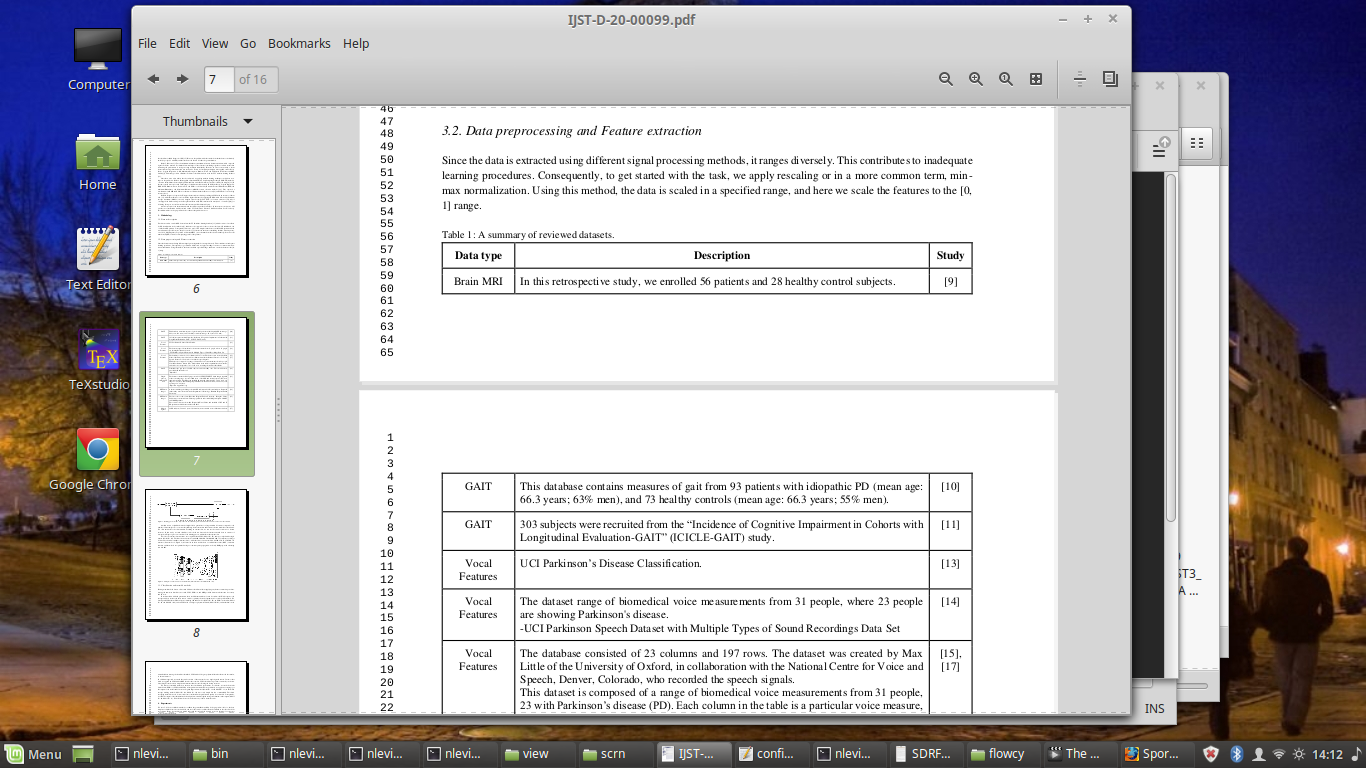
\includegraphics[trim=14cm 1.5cm 12cm 3cm,clip,width=.8\textwidth]{./scrn/s1.png}};

\rectann{darkRed}{0.7}{.5mm}{grammarArrowColor}{0.5}{4.9,-6.7}{1.5}{10.35}{1.15}

\node [anchor=west,bottom color=yellow!30!blue,top color=pink!70!green, 
inner sep=3, shading angle=50, text width=3cm]
  (longnote) at (7, 0) {\vspace{-8pt}%  %{\color{rb!85!red}{
{\cframedboxx{0mm}{2pt}{\large\raggedright\textbf{The authors provide 
citations for data sets used in their analyses ...}}}};

\end{tikzpicture}
\caption{Table Listing Analyzed Data Sets in the Parkinson's Article}
\label{fig:s1}
\end{figure}
  
\p{The authors summarize the data sets in a table within the main text 
(see Figure~\ref{fig:s1} here) and, in their bibliography, they 
cite these data sets either directly or by 
referencing publications where the relevant data sets are described 
(see Figure~\ref{fig:s2} here).  This properly 
credits authorship to the researchers who curated the data sets, and it gives readers a 
means to locate the raw data.  However, accessing and working with the raw data is 
inconvenient from a reader's point of view without most or all of the data sets being 
repackaged into a single archive that could be hosted and downloaded as a unit.  
Obtaining raw data from the resources identified in the bibliography requires 
several steps --- for instance, the PhysioNet sensor data can be downloaded 
as a zipped folder, while the demographic data attached to it has to be downloaded 
separately.  Some of the information obtained from \MRI{} and speech analysis 
(reported in papers cited as data sources for the primary article) is provided 
as supplemental materials within the secondary papers, which requires readers 
to browse through the articles so as to find downloadable links.  In short, piecing all 
the source data together forces readers to manually inspect multiple web resources 
and to manually interconnect files once they are downloaded.}

\p{Another complicating factor is that certain information present in the data sets 
is implicit within how the data sets are organized, requiring extra effort to 
extract this information in a machine-readable manner.  For instance, the PhysioNet 
sensor data uses a file-naming convention which encodes several pieces of 
information in the file names, such as whether the file presents a Parkinson's patient 
or a control subject.  By examining file names, it would be possible to construct a 
table with additional information providing context for the file contents.  However, 
such information is not directly included within the PhysioNet data set; it 
needs to be extracted by computer code.}

\begin{figure}
\begin{tikzpicture}
\node[inner sep=0pt] (bib) at (0,0)
    {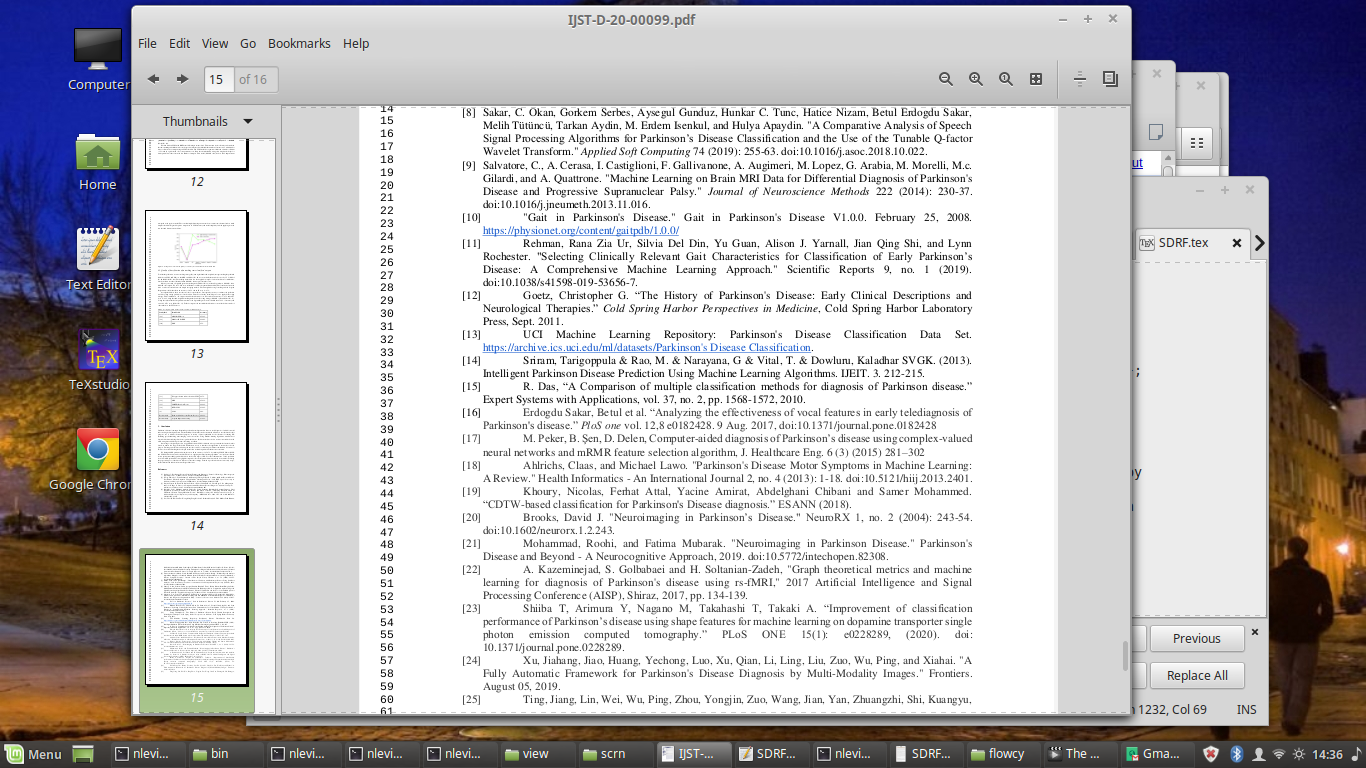
\includegraphics[trim=14cm 1.5cm 12cm 3cm,clip,width=.8\textwidth]{./scrn/s2.png}};
\ann{blue!50!orange}{1}{.6mm}{BlueGreen!90!red}{0.5}{-3.2,4.2}{2.8}{1}{1.1}
\ann{blue!50!orange}{1}{.6mm}{BlueGreen!90!red}{0.5}{-1,1.2}{5.2}{0.6}{1.1}

\colorarr{>=latex, ->}{fcBoxColor!60!black}
{0.8}{blGreen!30!red}{1}{1mm}{8,3}{4,1.5}

\colorarr{>=latex, ->}{fcBoxColor!60!black}
{0.8}{blGreen!30!red}{1}{1mm}{8,3}{-1.8,3.2}

\end{tikzpicture}
\caption{Bibliography (With Data Set Hyperrefs) in the Parkinson's Article}
\label{fig:s2}
\end{figure}

\p{This collection of data sets serves as an example of how technologies such 
as \SDRF{} can make scientific data more \q{FAIR} (Findable, Accessible, 
Interoperable, Reusable).  When the forthcoming article is published 
in the International Journal of Speech Technology, the disparate open-access 
data from the article's secondary sources will be provided as a single 
\SDRF{} archive.  This archive will provide machine-readable access to 
information spread across multiple sources, translated into a common file-format.  
In general, \SDRF{} encourages and implements features to help data sets 
conform to \FAIR{} and related standards, such as (1) bundling multiple data sets 
into a single archive; (2) migrating data to general-purpose representations 
wherever possible --- formats such as \XML{}, \HDFFive{}, \ARFF{}, or 
\DICOM{}; (3) providing meta-data in several formats, such as 
Research Objects, schema.org/Dataset, Digital Curation Center, \SciData{}, 
\BioCoder{}, and \MIBBI{} (Minimum Information for Biological and Biomedical 
Investigations); (4) identifying one or more \q{preferred applications} 
for examining/reusing the published data; (5) explicitly 
representing information encoded via file-names; 
(6) bundling raw data, meta-data, and (where possible) machine-readable 
article text into a single resource, which \SDRF{} calls a 
\q{Supplemental Archive;} and (7) annnotating the data sets to support 
microcitations granularly linking the publication to its associated 
Supplemental Archive.} 

\p{An important question for any \SDRF{} archive is how researchers 
will productively access the data once a Supplemental Archive has been 
downloaded.  Unlike the Flow Cytometry use-case discussed below, the 
Parkinson's archive spans several scientific disciplines, and 
there is no obvious application which could be preferred by default 
for examining the data files.  As a fallback option, \SDRF{} is 
designed to present data sets via \Qt{} Creator, a \Cpp{} Integrated 
Development Environment associated with the \Qt{} application-development 
framework.  \lSDRF{} includes code libraries to represent 
research meta-data as \Cpp{} objects, and these libraries can be 
opened as \Qt{} projects.  These may be 
supplemented with separate libraries extracting and 
managing information specific to individual data sets.  In 
particular, the Supplemental Archive for the forthcoming Parkinson's 
article will provide \Cpp{} classes encapsulating spreadsheet-like 
data (whether originally in \textbf{.xls}, \CSV{}, or space-delimited formats) 
republished in the unified data set.}

\p{An additional concern for \SDRF{} archives is how to properly annotate 
publications and data sets side-by-side.  In the Parkinson's article, 
individual \Cpp{} classes encapsulating tabular data serve as 
convenient microcitation targets: annotations within the relevant 
\Cpp{} code represent anchors through which the data set may be 
referenced (on a more precise scale than merely referencing the 
Supplemental Archive as a whole).  In some cases, individual 
class attributes can also be linked to lines in the authors' 
Python source code.  On the text side, certain individual 
paragraphs within the Parkinson's article specifically discuss individual 
data sets that the authors analyzed, the same data which the \SDRF{} 
archive encodes via \Cpp{} classes.  Therefore, those paragraphs 
can be cleanly linked to the corresponding \Cpp{} code annotations.  
This illustrates \SDRF{}'s recommended annotation/microcitation 
system, where segments in publication texts (identified for 
instance via \LaTeX{} \textbf{phantomsection} commands or 
\JATS{} \textbf{statement} tags) are linked to annotations or 
comments in code and/or raw data files in the Supplemental 
Archive.}

\section{Second Case Study: ``Marked T cell activation, senescence, exhaustion and skewing towards TH17 in patients with COVID-19 pneumonia'' from nature.com, 2020} 

\p{This article presents a use-case with some noteworthy contrasts to 
the Parkinson's publication described in the previous section.  The 
Covid-19 paper (\bhref{https://www.nature.com/articles/s41467-020-17292-4}) 
was published along with two data sets comprising Flow Cytometry Standard 
(\FCS{}) files hosted via the Flow Repository (\bhref{http://flowrepository.org/id/FR-FCM-Z2N4} 
and \bhref{http://flowrepository.org/id/FR-FCM-Z2N5}).  Links to the 
data sets (via \textbf{flowrepository.org} pages) are explictly provided 
in the publication's \q{Data Availability} section.  However, researchers 
still need to perform several steps to manually download the full set 
of relevant \FCS{} and meta-data files.}

\p{One feature of this second use-case is that the technical information 
in the data sets belong to a single scientific area (Flow Cytometry) 
and are encoded in a single format (\FCS{}).  As such, it is 
straightforward to identify the kind of software which 
researchers need to use to visualize the raw data --- any 
application which can parse \FCS{} files.  There are a variety 
of commercial as well as open-source Flow Cytometry applications 
which can be used to access \FCS{} data.  Once readers have 
downloaded the Flow Repository archives, then, they may individually 
load the \textbf{.fcs} files to study data which, in the 
original article, is summarized via figure illustrations.}

\p{This workflow nonetheless requires researchers to perform several 
manual steps before being able to use the published data.  The 
core problem is that existing Flow Cytometry software does not 
intrinsically have capabilities to read \PDF{} files, locate 
\FCS{} data sets, and interoperate with hosting platforms such 
as Flow Repository.  Employing this use-case as an example with 
which to demonstrate proper alignment between document viewers, 
publication/date repositories, and scientific software, 
Linguistic Technology Systems is developing a new 
Flow Cytometry application which \textit{can} interoperate with 
\PDF{} viewers and \SDRF{} archives.  This application is 
designed so that, when authors are reading a \PDF{} file 
associated with an \FCS{} data set, the \PDF{} viewer 
can automatically launch and signal to the \FCM{} application 
when a reader wishes to download and visualize \FCS{} files.  
In short, the \FCM{} application --- having received 
data from a \PDF{} viewer which implements an 
\SDRF{} inter-application protocol --- will automatically 
preform download and extraction steps that scientists 
otherwise would have to perform manually.}

\p{Note also that, although most of the relevant 
data for this Covid-19 article is in \FCS{} form, 
there is also supplemental clinical information provided 
in other formats.  For cases such as these, 
the LTS \FCM{} software includes code libraries allowing 
researchers to parse non-\FCS{} data as well in standard 
formats such as \XML{}, \HDFFive{}, or \ARFF{}.}  
   
\p{This use-case illustrates a general principle, that 
research data is most convenient for scientists when 
it is deployed within an infrastructure where 
portals, document viewers, and scientific applications 
may seamlessly interoperate.  Wherever possible, 
when they are reading published books or articles, 
researcher should be able to automatically launch 
the proper scientific application, download data 
sets, and examine raw data files in the preferred 
software with only one or two clicks --- instead 
of manually finding, downloading, merging/extracting, 
and then opening data files, these steps should be 
performed automatically as much as is feasible.}

\section{Conclusion}
\p{The two use-cases considered here are similar in that 
each concern articles which are linked to multiple data sets, 
and for maximum convenience it is optimal for researshers 
to be able to access this data without performing 
manual download andd merging/extracting actions.  
There are also some differences: in particular, the 
Parkinson's data spans multiple disciplines, whereas the 
Covid-19 data is more rigorously grounded in Flow Cytometry.  
As such, the operational requirements for the Covid-19 data, 
from a reader's point of view, are more clearly delineated: 
effective integration between the publication and its 
concomitant data sets is defined by launching Flow Cytometry 
software while a researcher is reading the publication, 
allowing the researcher to view the data via software 
similar to that used to generate/analyze the data 
while the reported research was being conducted.  In 
the case of the Parkinson's data, there is no single 
application which would seamlessly display the specrum 
of information considered in that article; as 
mentioned above, \SDRF{} defaults to using 
\Qt{} Creator as a fallback for loading Supplemental 
Archives where no other software is available.}

\p{Whether using \Qt{} Creator or a domain-specific application, 
it is preferable that each \SDRF{} archive be associated 
with one or more applications that researchers can use 
to view data (and extract information) from the archive.  
Moreover, these applications would ideally be linked 
to document viewers and also to publisher's portals, 
so that readers can automatically launch preferred 
applications and view Supplemental Archives while 
reading concordant publications.  In order to achieve 
this, scientific applications need to be augmented 
with plugins to parse \SDRF{} data.  In addition, 
we are developing an inter-application messaging protocol 
so that disparate applications with \SDRF{} plugins 
may interoperate.  In particular, \PDF{} viewers may 
interoperate with scientific applications so that 
publications' data sets may be automatically downloaded 
and visualized via the preferred software.}

\p{Our prototype example for an application utilizing such 
plugins, as mentioned above, will be software for 
Flow Cytometry.  We are also working on a \Qt{} Creator 
plugin so that \Qt{} Creator (as the \q{default} \SDRF{} 
software) can participate in \SDRF{} networks using the 
same protocol.  We will then expand the scope of 
this protocol via plugins for software concerning 
implementation such as image-analysis, molecular visualization, 
radiology, \ThreeD{} graphics, and so forth.}

\p{}
}
\end{document}



